\documentclass{beamer}
\usepackage[utf8]{inputenc}
\usepackage{amsmath}
\usepackage{amsfonts}
\usepackage{amssymb}
\usepackage{makeidx}
\usepackage{graphicx}
\usepackage{lmodern}
\usepackage{color}
\usepackage{xcolor}
\usepackage{bussproofs}
\usepackage{lscape}
\usepackage{listings}
\usepackage{amsthm}
\usetheme{CambridgeUS}

\usefonttheme{serif}

\title{Symbolic Execution Engine}
\author{Mudathir Mahgoub}
  
 
\begin{document}
 
\frame{\titlepage}
 
\begin{frame}
\frametitle{Symbolic Execution Engine}

\end{frame}

\begin{frame}
\frametitle{Software components}
\begin{figure}
 \centering
 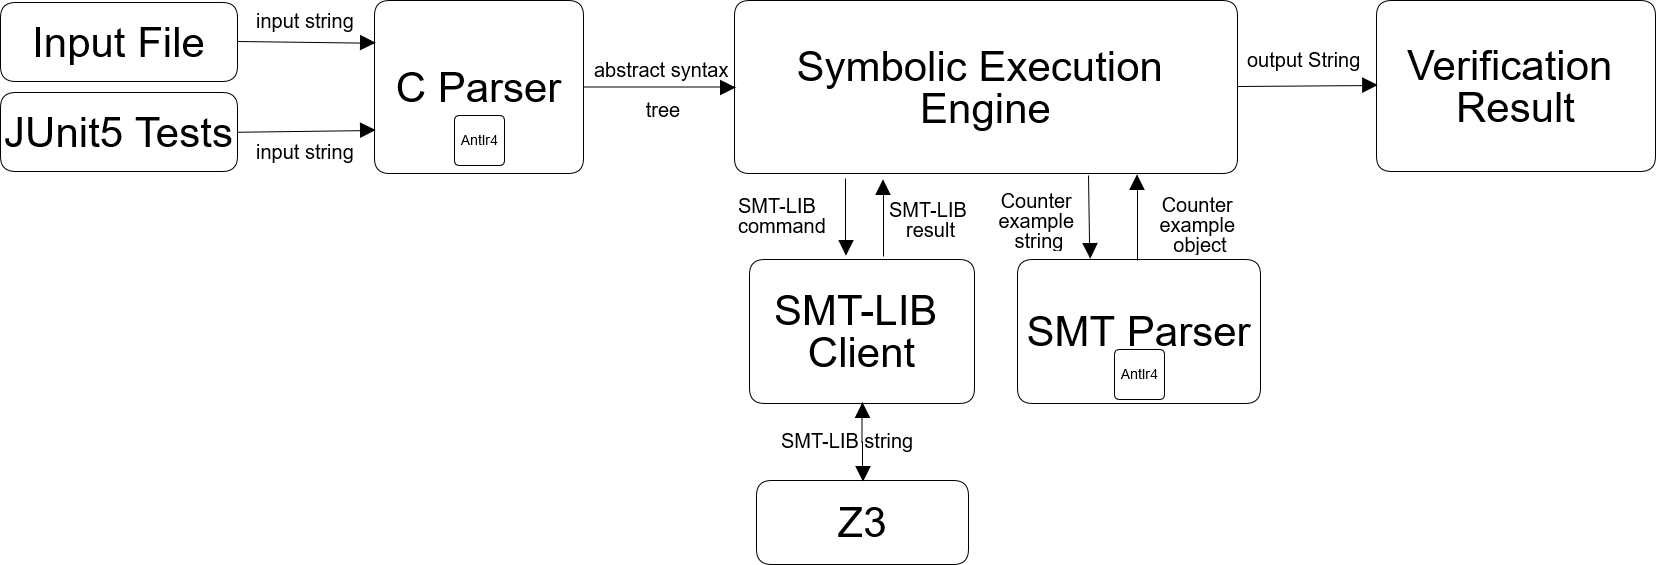
\includegraphics[scale=.18,keepaspectratio=true]{./engine.png}
\end{figure}
\end{frame}

%\definecolor{light-gray}{gray}{0.95}
%\lstset{backgroundcolor= \color{light-gray}}

\begin{frame}[fragile]
\frametitle{Execution}
\scriptsize

\begin{block}{Input: test.txt}
\begin{lstlisting}
SubBase(bool, int);
. |- \lambda x. \lambda y. (x y)[bool]: (int ->T) -> (bool -> T);
\end{lstlisting}
\end{block}

\begin{block} {Output: java -jar TypeChecker.jar -i test.txt}
\begin{lstlisting}
Yes
                        	SubBase(bool, int)
-------------------(var)	-------------------(subBase)
x: bool |- x : bool			bool <: int
--------------------------------------(subsumption)
x: bool |- x : int
\end{lstlisting}
\end{block}

\end{frame}


\begin{frame}[fragile]
\frametitle{Execution}
\scriptsize

\begin{block}{Input: test.txt}
\begin{lstlisting}
SubBase(bool, int);
. |- \lambda x. \lambda y. (x y)[bool]: (int ->T) -> (bool -> T);
\end{lstlisting}
\end{block}

\end{frame}

\end{document}
